\documentclass[aspectratio=169]{beamer}
\usepackage{xcolor}
\usepackage{multicol}
\usepackage{hyperref}
\usepackage{amsmath}
\usepackage{mhchem}
\usepackage{subcaption}
\usepackage{xparse}
\usepackage{physics}
\usepackage[mathscr]{euscript}  % \mathscr
\usepackage[style=verbose, backend=biber]{biblatex}

% Metadata of the presentation
\title{Phase Transitions in the Bose-Hubbard Model}
\subtitle{An in Depth Study of the Mott-Insulator to Superfluid Transition}
\author[DB]{Xeno De Vriendt, Robbe Brants}
\date{\today}


% Macro aimed at loading themes in different directories
\makeatletter
  \def\beamer@calltheme#1#2#3{%
    \def\beamer@themelist{#2}
    \@for\beamer@themename:=\beamer@themelist\do
    {\usepackage[{#1}]{\beamer@themelocation/#3\beamer@themename}}}

  \def\usefolder#1{
    \def\beamer@themelocation{#1}
  }
  \def\beamer@themelocation{}

% Load the UGent theme
\usefolder{./theme}
\usetheme[language=en,faculty=we,usecolors]{ugent}
\useinnertheme{ugent}
\useoutertheme{ugent}
\usecolortheme{ugent}
\usefonttheme{ugent}

% Path to images
\graphicspath{{./theme/}}

\bibliography{presentation.bib}


% Have this if you'd like section slides 
\AtBeginSection[]{
    \sectionframe
}

% \NewDocumentEnvironment{itemizewithimage}{ m b }{%
% \begin{center}%
%     \includegraphics[height=4cm,width=\textwidth,keepaspectratio]{#1}%
% \end{center}%
% \vfill%
% \begin{minipage}[t][3cm][t]{\textwidth}
%   \begin{itemize}%
%       #2
%   \end{itemize}%
% \end{minipage}
% }{%
% }
\definecolor{ugent_blue}{RGB}{30, 100, 200}
\renewcommand\emph[1]{\textcolor{ugent_blue}{\textbf{#1}}}

\begin{document}

\titleframe

\begin{frame}
  \frametitle{The Hubbard model represents an optical lattice containing ultra cold atoms}
  making two coherent laser beams propagating in opposite directions interfere with each other.
    \begin{onlyenv}<1>
      \begin{figure}
        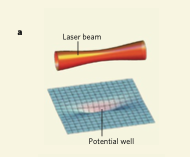
\includegraphics[scale=0.5]{../img/Optical-lattice-creation-a.png}
        \caption{Laser beam creates potential well \footcite{Greiner2008}.}
      \end{figure}
    \end{onlyenv}
    \begin{onlyenv}<2>
      \begin{figure}
        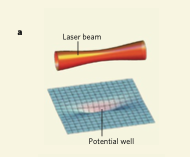
\includegraphics[scale=0.5]{../img/Optical-lattice-creation-a.png} 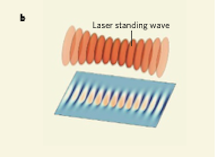
\includegraphics[scale=0.5]{../img/Optical-lattice-creation-b.png}
        \caption{Interference causes standing waves \footnotemark[1].}
      \end{figure} 
    \end{onlyenv}
    \begin{onlyenv}<3>
      \begin{figure}
        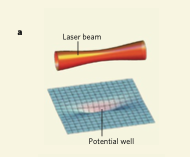
\includegraphics[scale=0.5]{../img/Optical-lattice-creation-a.png} 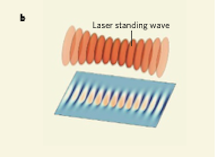
\includegraphics[scale=0.5]{../img/Optical-lattice-creation-b.png}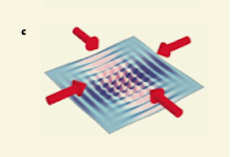
\includegraphics[scale=0.5]{../img/Optical-lattice-creation-c.png}
        \caption{Four such lasers create a lattice \footnotemark[1].}
      \end{figure} 
    \end{onlyenv}
\end{frame}

\begin{frame}
  \frametitle{Optical lattices containing super cold atoms closely resemble condensed matter physics
  }
  \begin{onlyenv}<1>
    \begin{figure}
      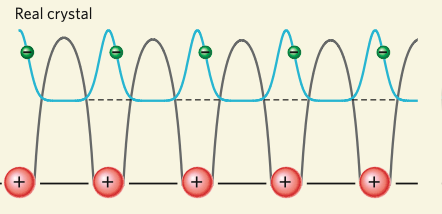
\includegraphics[scale=0.4]{../img/real-crystal.png}
      \caption{Potential well created by attractive electrostatic force between the electrons (–) and the ions (+) forming the crystal \footcite{Greiner2008}.}
    \end{figure}
  \end{onlyenv}
  \begin{onlyenv}<2>
    \begin{figure}
      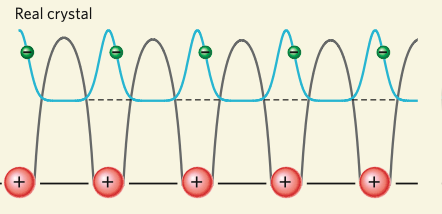
\includegraphics[scale=0.4]{../img/real-crystal.png} \\
      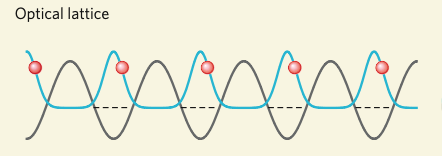
\includegraphics[scale=0.4]{../img/lattice.png}
      \caption{Simulated very well by an optical lattice \footnotemark[1].}
    \end{figure}
  \end{onlyenv}
\end{frame}

\begin{frame}
  \frametitle{Such lattices are indispensible in the study of different phases of matter}
  \begin{onlyenv}<1-3>
    \begin{columns}[T] % align columns
      \begin{column}{.48\textwidth}
        \begin{center}
          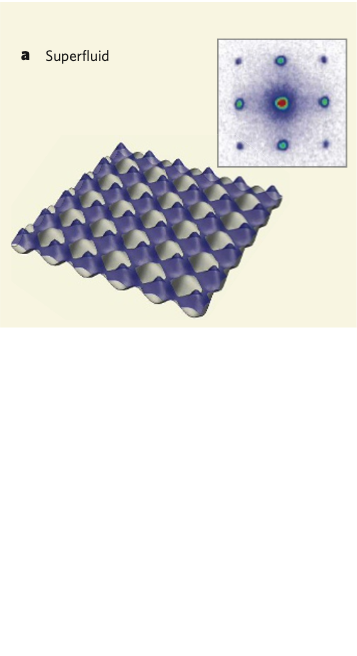
\includegraphics[scale=0.2]{../img/SF.png}
        \end{center}
      \end{column}%
      \hfill%
      \begin{column}{.48\textwidth}
        \begin{itemize}
          \item<2-> \textbf{Superfluid phase}
          \item<3-> Potential for single particle excitations independant from number of particles 
        \end{itemize}
      \end{column}%
    \end{columns}
  \end{onlyenv}
  \begin{onlyenv}<4->
    \begin{columns}[T] % align columns
      \begin{column}{.48\textwidth}
        \begin{center}
          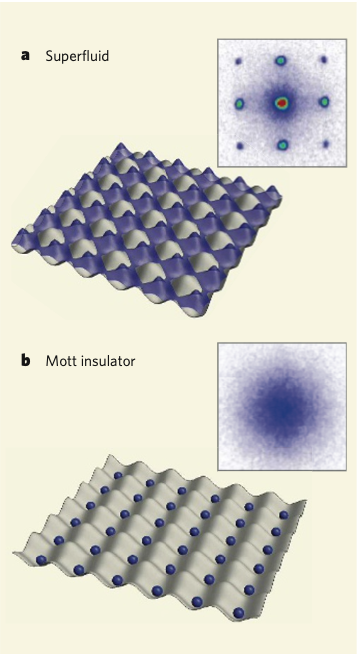
\includegraphics[scale=0.2]{../img/SF-MI.png}
        \end{center}
      \end{column}%
      \hfill%
      \begin{column}{.48\textwidth}
        \begin{itemize}
          \item<4-> \textbf{Superfluid phase}
          \item<4-> Potential for single particle excitations independant from number of particles
          \item<4-> \textbf{Mott-insulator phase}
          \item<5-> Strives for integer occupation in every potential well
        \end{itemize}
        \begin{alertblock}{Bose-Hubbard model}<6->
          Provides a relatively simpel theoretical model to simulate these phenomena.
        \end{alertblock}
      \end{column}%
    \end{columns}
  \end{onlyenv}
\end{frame}

\begin{frame}
\frametitle{Theory}
    Keep your theory short and to the point.
\end{frame}

\begin{frame}
\frametitle{Discuss your results.}
    \begin{itemize}
      \item Try to avoid text.
      \item Let your results speak for themselves.
    \end{itemize}
    
\end{frame}


\begin{frame}
\frametitle{Conclusions}
\begin{itemize}
  \item End your presentation with the most importatnt figures of your presentation.
  \item Mention possible future research routes.
\end{itemize}
\end{frame}

\end{document}
